\documentclass[12pt]{report}
\usepackage[a4paper,margin=1in]{geometry}
\usepackage[T1]{fontenc}
\usepackage[utf8]{inputenc}
\usepackage{lmodern}
\usepackage{microtype}
\usepackage{setspace}
\usepackage{amsmath,amssymb}
\usepackage{booktabs}
\usepackage{array}
\usepackage{tabularx}
\usepackage{ragged2e}
\usepackage{graphicx}
\usepackage{float}
\usepackage{caption}
\usepackage{enumitem}
\usepackage{xcolor}
\usepackage{hyperref}
\usepackage{tikz}
\usepackage[numbers]{natbib}

\usetikzlibrary{arrows.meta,positioning}
\hypersetup{colorlinks=true,linkcolor=blue,citecolor=blue,urlcolor=blue}
\setlength{\parindent}{0pt}
\setlength{\parskip}{0.55em}
\setlength{\emergencystretch}{2em}
\onehalfspacing
\captionsetup{font=small}
\newcolumntype{Y}{>{\RaggedRight\arraybackslash}X}
\newcommand{\assetroot}{thesis_report_assets}
\newcommand{\code}[1]{\texttt{#1}}
\newcommand{\insertassetfigure}[3]{%
\begin{figure}[H]
\centering
\IfFileExists{\assetroot/figures/#3}{\includegraphics[width=0.92\textwidth]{\assetroot/figures/#3}}{\fbox{\parbox[c][2.2in][c]{0.85\textwidth}{\centering Missing figure\\[0.3em]\code{\assetroot/figures/#3}}}}
\caption{#1}
\label{#2}
\end{figure}}

\begin{document}
\hypersetup{pageanchor=false}

\begin{titlepage}
\centering
{\Large National University of Singapore\par}
\vspace{1.5cm}
{\Huge\bfseries Intraday Implied-Volatility Curve Forecasting for Options Mispricing Detection\par}
\vspace{0.8cm}
{\Large Rewritten Thesis Report\par}
\vspace{2cm}
{\large James Shen\par}
{\large School of Computing\par}
\vfill
{\large April 2026\par}
\end{titlepage}

\pagenumbering{roman}
\chapter*{Abstract}
\addcontentsline{toc}{chapter}{Abstract}
This thesis studies short-horizon forecasting of the SPY implied-volatility (IV) curve rather than forecasting returns, realized volatility, or a single scalar IV measure. The forecasting target is a fixed seven-point moneyness grid in a single maturity bucket centered around 30 days to expiry. At each timestamp, the model predicts the next curve, compares it with the currently quoted curve, and interprets the discrepancy as a stylized options-mispricing signal. The practical question is whether a recurrent sequence model can recover short-horizon curve dynamics strongly enough to beat linear, econometric, tree-based, and coefficient-based baselines under temporally correct evaluation.

The final study is built around a 5-minute SPY dataset, a carry-forward curve-construction layer that densifies sparse option bars, an optional SVI smoothing variant, an overlap-safe walk-forward benchmark, and an execution-aware backtest with exposure limits and transaction frictions. The final carry benchmark contains 50,019 supervised samples and compares ten baselines, four LSTM variants, and four xLSTM variants on the same \code{seq12}, one-bar-ahead task. Under the standardized fixed-threshold benchmark, Elastic Net is the best statistical model with RMSE 0.010886. After threshold sweeping the same standardized prediction paths to study economic calibration, xLSTM \code{b2/e256} becomes the best economic model with net PnL 0.121296 and Sharpe 3.876. In contrast, the retuned conventional LSTM family remains materially weaker and economically negative even after threshold filtering.

The thesis contribution is therefore not a blanket claim that recurrent models dominate all alternatives. The stronger finding is more nuanced: (i) careful curve construction and walk-forward evaluation are essential, (ii) sparse-linear and long-memory baselines remain extremely strong on IV-curve forecasting, and (iii) modern recurrence in the form of xLSTM can produce the strongest monetizable signal once the decision layer is economically filtered, even when a linear model still leads on point forecast accuracy. An SVI sensitivity study further shows that improved smile fitting does not automatically improve the final ranking.

\tableofcontents
\clearpage
\pagenumbering{arabic}
\hypersetup{pageanchor=true}

\chapter{Introduction}

\section{Why short-horizon IV forecasting matters}
Options are quoted, compared, and risk-managed in implied-volatility space. For that reason, the object that traders and volatility desks actually inspect is not only the option premium itself, but the shape of the IV curve across moneyness and maturity. Forecasting the curve directly is therefore more structurally aligned with options trading than forecasting a single volatility scalar or a raw option return. Earlier work on IV dynamics showed that volatility surfaces have systematic structure rather than behaving like independent cross-sectional noise \citep{cont2002dynamics}. Later work also showed that predictable IV-surface dynamics can translate into economically meaningful signals \citep{bernales2014,borochin2025}.

This thesis focuses on the most demanding version of that problem: next-tick intraday forecasting of a fixed-maturity IV curve. The target horizon is only one 5-minute bar ahead in the final benchmark. That setting is interesting because it is close to the time scale at which an options-mispricing signal would have to be acted upon, but it is also difficult because the signal is weak, option bars are sparse, and transaction costs can erase apparent improvements very quickly.

\section{Why the problem is still difficult}
Three frictions make this task harder than standard financial forecasting benchmarks.

First, the data object itself is awkward. Historical intraday option bars are sparse, especially away from the most active strikes, so a fixed-grid curve has to be reconstructed from an incomplete traded cross-section. That makes curve construction a first-order research problem rather than a preprocessing footnote. The literature on arbitrage-aware surface fitting, including SVI-based approaches, makes clear that shape quality matters \citep{gatheral2014arbitrage}.

Second, strong baselines are easy to underestimate. Simple autoregressive, sparse-linear, and long-memory models often remain competitive in volatility forecasting \citep{engle1982,bollerslev1986,corsi2009}. More recent IV-surface work also shows that basis-and-coefficient approaches and tree-based models can be very strong competitors \citep{chen2024bspline}. Any deep-learning claim should therefore be made only after the baseline library is already difficult to beat.

Third, evaluation protocol matters as much as model class. A model that looks attractive on one split can weaken under expanding-window retraining, common-window standardization, or explicit execution frictions. Recent critical reviews of IV forecasting warn that leakage, weak temporal splits, and overly favorable feature design can make complex models look stronger than they really are \citep{arratia2025}. This thesis is built around that warning.

\section{Thesis statement and contributions}
The central claim of the thesis is deliberately narrower than ``deep learning beats classical models.'' The claim is:

\begin{quote}
A carefully retuned xLSTM can produce the strongest threshold-filtered trading signal on the final intraday carry-forward benchmark, but sparse-linear and long-memory baselines remain stronger on raw point forecast accuracy, and that distinction only becomes visible under a strict walk-forward and execution-aware evaluation pipeline.
\end{quote}

The main contributions are fourfold.
\begin{enumerate}[leftmargin=1.3cm]
    \item A reproducible end-to-end IV-curve forecasting pipeline that starts from option bars and ends with statistically and economically evaluated signals.
    \item A final 5-minute benchmark built on a denser carry-forward panel, a broad model library, overlap-safe walk-forward stitching, and standardized backtesting.
    \item A modern recurrent extension using xLSTM, tested against conventional LSTM and strong non-neural baselines under the same protocol.
    \item A focused sensitivity study showing that SVI smoothing improves structural curve fitting but does not overturn the downstream model ranking.
\end{enumerate}

\chapter{Literature Review}

\section{From option prices to implied-volatility geometry}
The intellectual starting point is the observation that options are more naturally compared in volatility space than in premium space. Work on IV-surface dynamics established that the smile and surface exhibit systematic movement, common factors, and persistence \citep{cont2002dynamics}. Later evidence showed that surface predictability can have economic value, especially when cross-surface information is exploited rather than only local node dynamics \citep{bernales2014}. Related work on factor-style surface models, including Nelson--Siegel-type representations, further suggests that a large share of smile movement can be described through a small number of latent shape components \citep{kearney2019}.

That line of literature is important for this thesis because it motivates two design principles. The first is that the IV curve should be treated as a structured object rather than as seven unrelated regressions. The second is that model comparisons should include structure-preserving baselines, not only pointwise autoregressions.

\section{How machine learning entered volatility and derivative modeling}
Machine learning has a long history in derivatives research. Early work by Hutchinson, Lo, and Poggio showed that learning-based methods could already be used for pricing and hedging derivatives \citep{hutchinson1994}. In the volatility literature, ARCH and GARCH established the importance of time-varying conditional variance \citep{engle1982,bollerslev1986}, while HAR-style models later provided a simple long-memory alternative that remains influential \citep{corsi2009}. These ideas still matter because they motivate several of the baselines used in this thesis.

Modern deep learning changed the style of the comparison rather than eliminating the older models. The original LSTM architecture was introduced to stabilize long-range sequence learning \citep{hochreiter1997}, and later financial work showed that recurrent models can outperform simpler methods in some market-prediction tasks \citep{fischer2018}. More recent work such as xLSTM revisits recurrence with updated memory blocks and scaling behavior \citep{beck2024xlstm}. In parallel, IV-specific applied work and hybrid GARCH--LSTM discussions motivated the initial decision to test sequence models in an options setting \citep{hull2019framing,sullivan2019lstm,zhao2024garchlstm}.

\section{What the recent IV literature still does not test enough}
Recent IV-surface papers have improved the structural side of the problem. Chen, Li, and Yu forecast B-spline coefficients with tree-based machine learning, showing that coefficient prediction can be a serious alternative to direct node forecasting \citep{chen2024bspline}. Borochin and Zhao emphasize that economic value must be distinguished from pure forecast improvement \citep{borochin2025}. Arratia et al.\ add a strong methodological caution by showing how easily IV-forecasting claims can be overstated under weak protocol design \citep{arratia2025}.

What remains relatively under-tested is the combination of all of the following in a single study:
\begin{enumerate}[leftmargin=1.3cm]
    \item intraday data rather than daily or lower frequency data;
    \item a directly tradable fixed-maturity curve target instead of only coefficients or scalars;
    \item strong linear, tree-based, coefficient-based, and recurrent baselines in one benchmark;
    \item expanding-window retraining and overlap-safe stitching;
    \item an execution-aware economic layer that is strict enough to overturn weak signals.
\end{enumerate}

This thesis is designed around that combined gap rather than around the narrower claim of ``using LSTM for options.''

\chapter{Problem Formulation}

\section{Target object}
Let the fixed moneyness grid be
\[
\mathcal{M}=\{-0.15,-0.10,-0.05,0.00,0.05,0.10,0.15\}.
\]
For each timestamp \(t\), the observed IV curve is
\[
\mathbf{c}_t = \big[\sigma_t(m_1), \ldots, \sigma_t(m_7)\big]^\top \in \mathbb{R}^7,
\]
where \(\sigma_t(m_i)\) denotes the implied volatility at moneyness node \(m_i\) for a maturity bucket centered around 30 days to expiry.

The forecasting task is one-step-ahead curve prediction in the final benchmark:
\[
\hat{\mathbf{c}}_{t+1} = f_\theta(\mathbf{X}_t),
\]
where \(\mathbf{X}_t \in \mathbb{R}^{L \times d}\) is the sequence of the last \(L=12\) feature vectors and \(d\) is the feature dimension.

\section{Learning objective}
The supervised dataset is
\[
\mathcal{D}=\{(\mathbf{X}_t,\mathbf{c}_{t+1})\}_{t=L}^{T-1}.
\]
Models are trained to minimize a node-wise Huber loss,
\[
\mathcal{L}(\theta)=\frac{1}{N}\sum_{t}\sum_{j=1}^{7}\ell_\delta\!\left(\hat{c}_{t+1,j}-c_{t+1,j}\right),
\]
with optional smoothness and shape-projection hooks for the neural models. Forecast quality is evaluated by RMSE, MAE, \(R^2\), and region-level error decomposition.

\section{Signal rule}
The trading layer transforms the forecast error relative to the current curve into a scalar signal
\[
s_t = \sum_{j=1}^{7} w_j\big(\hat{c}_{t+1,j} - c_{t,j}\big),
\]
where \(w_j\) are nonnegative weights that approximate a vega-style aggregation across the curve nodes. A thresholded directional action is then defined as
\[
a_t =
\begin{cases}
1, & s_t > \tau, \\
-1, & s_t < -\tau, \\
0, & |s_t| \le \tau.
\end{cases}
\]
This action is held for one 5-minute bar in the final benchmark. The main economic outputs are net PnL, Sharpe, hit rate, and drawdown under explicit execution assumptions.

\chapter{Methodology}

\section{End-to-end data pipeline}
Figure~\ref{fig:pipeline} summarizes the workflow used in the final system.

\begin{figure}[H]
\centering
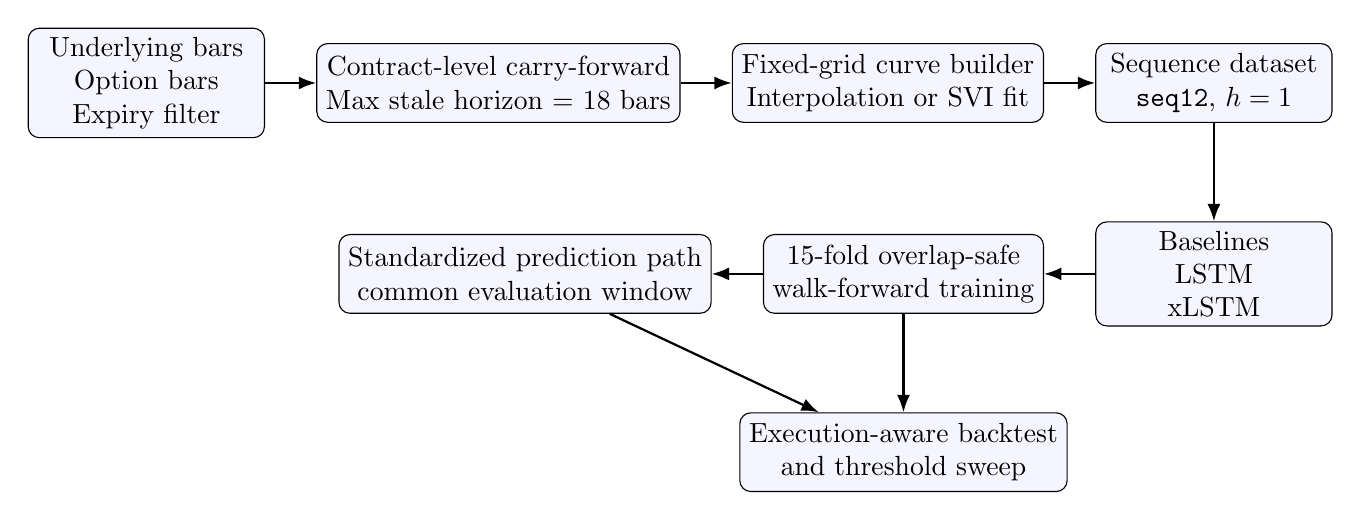
\begin{tikzpicture}[
    node distance=1.25cm and 0.65cm,
    box/.style={draw, rounded corners, align=center, minimum height=1.0cm, minimum width=3.0cm, fill=blue!4},
    arrow/.style={-{Latex[length=2.2mm]}, thick}
]
\node[box] (raw) {Underlying bars\\Option bars\\Expiry filter};
\node[box, right=of raw] (carry) {Contract-level carry-forward\\Max stale horizon = 18 bars};
\node[box, right=of carry] (curve) {Fixed-grid curve builder\\Interpolation or SVI fit};
\node[box, right=of curve] (dataset) {Sequence dataset\\\code{seq12}, \(h=1\)};
\node[box, below=of dataset] (models) {Baselines\\LSTM\\xLSTM};
\node[box, left=of models] (wf) {15-fold overlap-safe\\walk-forward training};
\node[box, left=of wf] (std) {Standardized prediction path\\common evaluation window};
\node[box, below=of wf] (bt) {Execution-aware backtest\\and threshold sweep};
\draw[arrow] (raw) -- (carry);
\draw[arrow] (carry) -- (curve);
\draw[arrow] (curve) -- (dataset);
\draw[arrow] (dataset) -- (models);
\draw[arrow] (models) -- (wf);
\draw[arrow] (wf) -- (std);
\draw[arrow] (wf) -- (bt);
\draw[arrow] (std) -- (bt);
\end{tikzpicture}
\caption{Final methodology pipeline. The benchmark starts from intraday market data, densifies sparse contracts through bounded carry-forward, constructs fixed-grid IV curves, trains each model with overlap-safe walk-forward retraining, and then evaluates both fixed-threshold and threshold-swept execution-aware signals.}
\label{fig:pipeline}
\end{figure}

\section{Curve construction}
The final panel uses a contract-level carry-forward layer before curve fitting. If a contract does not trade in a specific 5-minute bar, its last observed option value is carried forward on the trading calendar, up to a maximum staleness of 18 bars (90 minutes). This is materially different from carrying forward the already-fitted grid nodes: the fill happens at the contract level first, then the smile is reconstructed.

This design addresses the main empirical bottleneck in the raw 5-minute options panel. The problem was not missing timestamps but cross-sectional sparsity: many timestamps had too few traded strikes to identify the smile shape cleanly. The carry-forward layer raises the median number of usable moneyness points per timestamp from roughly two to roughly five, which is enough to make structure-aware fitting feasible in the SVI sensitivity.

\section{Model families}
The final benchmark includes three broad model groups.

\textbf{Classical and tabular baselines.} Persistence, AR(1) per grid point, factor AR/VAR, a GARCH-style ATM-shift model, Elastic Net, MLP, ExtraTrees, histogram gradient boosting, HAR factor forecasting, and a smile-coefficient baseline. These models were included because strong IV forecasting results are impossible to interpret unless sparse-linear, tree-based, and coefficient-based alternatives are already difficult to beat \citep{chen2024bspline,corsi2009}.

\textbf{Conventional LSTM.} The LSTM models use a sequence encoder with Huber loss, gradient clipping, early stopping, smoothness penalties, and optional shape projection. The retuned carry benchmark revisits the LSTM family with the stronger training budget that had been used in the earlier successful 5-minute experiments.

\textbf{xLSTM.} The xLSTM models use the official \code{mLSTM} block stack from \citet{beck2024xlstm}. In this environment the CUDA-only \code{sLSTM} path was not available, so the implemented extension uses the portable xLSTM configuration rather than the full GPU-only variant.

\section{Training and evaluation protocol}
The final benchmark uses the carry-forward dataset \code{spy\_5min\_walkforward\_h1\_dataset\_carry\_local.npz} with 50,019 supervised samples, sequence length 12, and horizon 1. The walk-forward split uses:
\begin{itemize}[leftmargin=1.2cm]
    \item initial train size: 17,630,
    \item validation size: 3,526,
    \item test size: 3,526,
    \item step size: 1,763,
    \item stitch mode: frontier.
\end{itemize}

This produces 15 expanding-window folds without double-counting timestamps in the stitched test path. The retuned neural runs use batch size 64, 40 maximum epochs, learning rate 0.001, and early stopping patience 8. These settings matter because the weaker carry benchmark that preceded the retune used a substantially lighter training budget and undertrained the recurrent models.

Two economic layers are reported. The first is a fixed-threshold standardized benchmark at \(\tau=0.0015\). The second is a threshold sweep over \(\tau \in \{0.0015, 0.0020, 0.0025, 0.0030, 0.0040, 0.0050, 0.0075, 0.0100\}\). The threshold sweep is performed on the standardized evaluation path itself, so it should be interpreted as an economic sensitivity study rather than as a completely separate out-of-sample calibration.

\chapter{Experiments}

\section{From pilot studies to the final benchmark}
The full empirical program moved through three stages.

\textbf{Stage 1: pipeline validation.} Daily and hourly pilot studies verified the provider abstraction, panel construction, baseline training, recurrent training, and backtest interfaces. These studies also revealed that low-sample settings strongly favored simple baselines.

\textbf{Stage 2: intraday model search.} The first 5-minute study established that richer intraday features and larger sample sizes make recurrent models much more competitive, but it also exposed a data-quality problem: the raw options panel was too sparse for robust curve fitting at many timestamps.

\textbf{Stage 3: final benchmark and sensitivity checks.} The final benchmark introduced contract-level carry-forward, overlap-safe walk-forward stitching, the broadened baseline library, the xLSTM extension, and the threshold-swept execution layer. This is the main experiment used for the thesis conclusion. The SVI version of the carry panel is then used as the principal curve-construction sensitivity test.

\section{System design and reproducibility}
The repository is organized around four layers:
\begin{enumerate}[leftmargin=1.2cm]
    \item provider and data engineering modules for underlying bars, option bars, carry-forward, and curve construction;
    \item dataset builders for fixed-grid supervised sequences;
    \item model modules for baselines, LSTM, and xLSTM;
    \item evaluation modules for walk-forward stitching, statistical testing, and backtesting.
\end{enumerate}

This architecture matters because it allows the thesis to change the data layer (for example, by adding carry-forward or SVI) without rewriting the rest of the training and evaluation stack.

\section{Main experiment: retuned carry benchmark}
The main experiment compares 18 models on the same standardized \code{seq12}, one-bar-ahead carry-forward benchmark:
\begin{itemize}[leftmargin=1.2cm]
    \item 10 baselines,
    \item 4 retuned LSTM variants,
    \item 4 retuned xLSTM variants.
\end{itemize}

The benchmark uses one seed, 15 walk-forward folds, one standardized prediction path, and the execution-aware configuration with 0.25 per-trade exposure, 0.05 minimum exposure, at most 8 concurrent positions, gross exposure cap 2.0, net exposure cap 1.0, and an effective 17 bps round-trip cost.

\section{Sensitivity experiment: carry plus SVI}
The main sensitivity experiment replaces the carry-only interpolation layer with carry plus SVI smoothing. This benchmark keeps the same 5-minute geometry, the same walk-forward protocol, and the same model families, but changes the way the curve is reconstructed once the densified contract panel is available. The question is not whether SVI is mathematically cleaner in isolation, but whether it improves the final forecasting and trading ranking on this dataset.

\chapter{Results and Analysis}

\section{Main benchmark: statistical leader versus economic leader}
Table~\ref{tab:main_results} presents the core result of the thesis. The fixed-threshold benchmark and the threshold-swept benchmark answer different questions. The fixed-threshold results show which model is the strongest pure forecasting system under one common execution rule. The threshold-swept results show which model becomes most economically attractive once the decision layer is filtered for high-confidence signals.

\begin{table}[H]
\centering
\caption{Main retuned carry benchmark on the standardized \code{seq12}, one-bar-ahead test path. The ``best threshold'' columns come from the descriptive threshold sweep on the same standardized path.}
\label{tab:main_results}
\small
\begin{tabularx}{\textwidth}{l c c c c c Y}
\toprule
\textbf{Model} & \textbf{Family} & \textbf{RMSE} & \textbf{Fixed net PnL} & \textbf{Best \(\tau\)} & \textbf{Tuned net PnL} & \textbf{Reading} \\
\midrule
ElasticNet & Baseline & 0.010886 & 0.100416 & 0.0025 & 0.110865 & Best statistical model; remains near the economic frontier. \\
xLSTM b2/e256 & xLSTM & 0.013914 & -0.004776 & 0.0050 & 0.121296 & Best tuned economic model; sparse, high-conviction signal. \\
MLP & Baseline & 0.012646 & 0.000977 & 0.0030 & 0.115634 & Strong nonlinear tabular benchmark. \\
HAR factor & Baseline & 0.013573 & 0.084505 & 0.0030 & 0.114551 & Strong long-memory benchmark. \\
Smile coefficient & Baseline & 0.020815 & 0.068293 & 0.0030 & 0.109536 & Best structure-preserving baseline economically. \\
LSTM 2x128 & LSTM & 0.033279 & -3.787900 & 0.0100 & -0.386723 & Retuning improved it, but it remained uncompetitive economically. \\
\bottomrule
\end{tabularx}
\end{table}

\insertassetfigure{Retuned carry benchmark trade-off between statistical accuracy and tuned economic value. ElasticNet remains the left-most point on RMSE, while xLSTM \code{b2/e256} becomes the highest point on tuned net PnL after threshold filtering. The conventional LSTM family remains far from this frontier.}{fig:tradeoff}{fig_carry_retuned_tradeoff.png}

Figure~\ref{fig:tradeoff} summarizes the central tension of the study. ElasticNet is still the best point forecaster, and the forecast-loss evidence remains strong enough that it should not be displaced as the statistical winner. However, once the standardized signal path is filtered through a stricter decision threshold, xLSTM \code{b2/e256} overtakes the baselines on net PnL. This is why the thesis distinguishes between a \emph{statistical leader} and an \emph{economic leader} rather than forcing a single metric to do both jobs.

The fixed-threshold and tuned-threshold results also explain why the retune mattered. Under the weaker carry benchmark, the recurrent models were undertrained and often overtraded. With the stronger training budget, xLSTM moves into the same region of the trade-off frontier as the strongest baselines. The conventional LSTM family improves materially in RMSE relative to its weak-budget version, but it still generates too many low-quality trades and remains negative even after thresholding.

\section{Why the xLSTM result matters}
The best tuned xLSTM is not merely ``less bad'' than the old LSTM. It is qualitatively different in how it trades. The best xLSTM threshold is 0.0050, far stricter than the fixed benchmark threshold of 0.0015. Under that rule it takes only 88 trades across 28,208 evaluation periods and achieves Sharpe 3.876. The best plain LSTM, by contrast, still requires a threshold of 0.0100 and remains negative after 1,235 trades. The practical interpretation is that the xLSTM is not winning by producing more signals. It is winning by producing fewer, more selective signals.

\insertassetfigure{Thresholded xLSTM equity curve on the final retuned carry benchmark. The figure uses the best xLSTM configuration (\code{b2/e256}) and its best descriptive threshold (\(\tau=0.0050\)). The key point is not that the equity path is spectacular in absolute size, but that it is smoother and more selective than the conventional LSTM alternatives under the same execution layer.}{fig:xlstm_equity}{fig_xlstm_thresholded_equity_curve.png}

Figure~\ref{fig:xlstm_equity} should be read together with Table~\ref{tab:main_results}. The xLSTM does not beat ElasticNet on RMSE, and the thesis should not claim that it does. What the figure shows is that once the objective shifts from point forecast error to monetizable mispricing detection, the xLSTM becomes the strongest model in the experiment. That is the core reason to keep a modern recurrent architecture in the final model comparison.

\section{Sensitivity to SVI smoothing}
The SVI sensitivity is useful precisely because it separates two issues that are often conflated: structural curve fitting and downstream signal quality. Carry-forward makes SVI operational on most slices, but the downstream benchmark still does not improve.

\insertassetfigure{Fit-method mix in the SVI carry panel. Contract-level carry-forward makes direct SVI fitting feasible on 92.8\% of rows, so the weak SVI result is not caused by an inability to fit the smile at all.}{fig:svi_fit_mix}{fig_svi_carry_fit_mix.png}

Figure~\ref{fig:svi_fit_mix} shows that the SVI panel is structurally meaningful: 46,427 of 50,031 rows are direct SVI fits, only 2,760 rows fall back to interpolation, and 844 rows still require flat fill. In other words, carry-forward solves enough of the sparsity problem to make SVI feasible on the large majority of the panel.

Yet the completed SVI benchmark does not improve the final model ranking. In the no-SVI carry benchmark, ElasticNet achieves RMSE 0.010886 and xLSTM \code{b2/e256} achieves RMSE 0.015034. In the SVI benchmark, those values worsen to 0.015476 and 0.019468 respectively. Economically, ElasticNet remains the winner in the SVI run, while xLSTM remains the best neural model but falls further behind. This means that cleaner smile fitting does not automatically create a better forecasting target. On this dataset, the signal bottleneck remains the tradability and calibration of the predicted curve changes, not only the smoothness of the curve-construction layer.

\section{Statistical checks and what they imply}
The thesis still needs a statistical reading alongside the economic one. In the carry-versus-SVI family comparisons, pairwise Diebold--Mariano tests consistently favor ElasticNet over the recurrent alternatives. In the carry benchmark, ElasticNet beats xLSTM \code{b2/e256} with overall DM statistic \(-19.73\) and \(p=0.0\). In the SVI benchmark, the same comparison strengthens to \(-24.18\) with \(p=0.0\). The correct interpretation is therefore not that xLSTM has become the statistically best model. It has become the strongest \emph{economically filtered} model, while ElasticNet remains the strongest \emph{forecast-loss} model.

That distinction is central to the thesis. If the objective is pure point forecast accuracy, the best answer remains sparse linear modeling. If the objective is a thresholded mispricing signal under the execution layer used here, the xLSTM becomes the most attractive model. Both facts should appear in the final conclusion.

\chapter{Discussion and Future Work}

\section{What the study establishes}
The study establishes five main points.

\begin{enumerate}[leftmargin=1.3cm]
    \item Short-horizon IV-curve forecasting is highly sensitive to data engineering. Carry-forward was not a cosmetic improvement; it was necessary to make the intraday panel dense enough for serious modeling.
    \item Strong baselines remain essential. ElasticNet, HAR, MLP, and smile-coefficient forecasting all remain close to the frontier, and any neural claim that ignores them would be weak.
    \item Conventional LSTM does not survive the final benchmark cleanly. Even after a stronger training budget, it remains miscalibrated economically.
    \item xLSTM is materially better than the conventional LSTM family on this task. It does not displace ElasticNet statistically, but it becomes the best tuned economic model on the final carry benchmark.
    \item SVI improves structural smile fitting but does not, by itself, solve the downstream forecasting problem.
\end{enumerate}

Taken together, these findings support a more precise thesis claim than the one the project started with. The contribution is not ``LSTM beats classical models.'' The contribution is that intraday IV-curve forecasting should be judged on both statistical and economic dimensions, and that the strongest modern recurrent model can win on the economic dimension only after careful data engineering and signal filtering.

\section{Limitations}
The final report should still state the remaining limitations clearly.

\begin{enumerate}[leftmargin=1.3cm]
    \item The final retuned carry benchmark is single-seed. Earlier parts of the project used multi-seed comparisons, but the strongest retuned carry benchmark remains computationally expensive.
    \item The threshold sweep is descriptive on the evaluation window itself. It demonstrates calibratability of the signal, but it is not a fully separated production threshold-selection experiment.
    \item The economic layer is execution-aware but still stylized. It is not a contract-level order-book simulator and it does not hold options to expiry.
    \item The study uses one underlying and one maturity bucket. Broader cross-asset and cross-maturity validation remains open.
    \item The SVI sensitivity was run as a curve-construction test rather than a fully retuned architecture benchmark. It is therefore best interpreted as evidence about the data layer, not the final neural hyperparameter frontier.
\end{enumerate}

\section{Future work}
The most natural extensions follow directly from the limitations.

First, the economic layer should be made stricter by separating threshold selection from the final evaluation window and by moving from a curve-level pseudo-portfolio toward a more realistic option-position simulator. Second, the structure-aware route should be pushed further by comparing direct node forecasting with explicit coefficient forecasting or SVI-parameter forecasting, rather than using SVI only as a preprocessing sensitivity. Third, the xLSTM result deserves a small multi-seed follow-up, because it is now the strongest economic model in the benchmark and should be stress-tested on seed stability. Fourth, the same carry-forward benchmark should be extended to additional liquid underlyings and multiple maturity buckets.

\section*{Closing summary}
The rewritten thesis story is therefore straightforward. Earlier pilot studies established that the problem was real but hard, and that simple baselines dominate low-sample settings. The final 5-minute carry-forward benchmark then showed that strong baselines still win on RMSE, but that a modern recurrent model---xLSTM \code{b2/e256}---produces the best threshold-filtered economic outcome once the problem is judged as a mispricing-detection task rather than as pure point forecasting. That is a narrower claim than ``deep learning wins,'' but it is also a more credible and more useful one.

\begin{thebibliography}{99}

\bibitem{arratia2025}
Arratia, A., El Daou, M., Kagerhuber, J., and Smolyarova, Y. (2025).
\newblock Examining challenges in implied volatility forecasting: A critical review of data leakage and feature engineering combined with high-complexity models.
\newblock \emph{Computational Economics}.

\bibitem{beck2024xlstm}
Beck, M., P\"oppel, K., Spanring, M., Auer, A., Prudnikova, O., Kopp, M., Klambauer, G., Brandstetter, J., and Hochreiter, S. (2024).
\newblock xLSTM: Extended Long Short-Term Memory.
\newblock arXiv preprint arXiv:2405.04517.

\bibitem{bernales2014}
Bernales, A. and Guidolin, M. (2014).
\newblock Can we forecast the implied volatility surface dynamics of equity options? Predictability and economic value tests.
\newblock \emph{Journal of Banking \& Finance}, 46, 326--342.

\bibitem{bollerslev1986}
Bollerslev, T. (1986).
\newblock Generalized autoregressive conditional heteroskedasticity.
\newblock \emph{Journal of Econometrics}, 31(3), 307--327.

\bibitem{borochin2025}
Borochin, P. and Zhao, Y. (2025).
\newblock The economic value of equity implied volatility forecasting with machine learning.
\newblock \emph{Journal of Empirical Finance}, 82.

\bibitem{chen2024bspline}
Chen, Z., Li, Y., and Yu, C.~L. (2024).
\newblock Modeling implied volatility surface using B-splines with time-dependent coefficients predicted by tree-based machine learning methods.
\newblock \emph{Mathematics}, 12(7), 1100.

\bibitem{cont2002dynamics}
Cont, R. and da Fonseca, J. (2002).
\newblock Dynamics of implied volatility surfaces.
\newblock \emph{Quantitative Finance}, 2(1), 45--60.

\bibitem{corsi2009}
Corsi, F. (2009).
\newblock A simple approximate long-memory model of realized volatility.
\newblock \emph{Journal of Financial Econometrics}, 7(2), 174--196.

\bibitem{diebold1995}
Diebold, F.~X. and Mariano, R.~S. (1995).
\newblock Comparing predictive accuracy.
\newblock \emph{Journal of Business \& Economic Statistics}, 13(3), 253--263.

\bibitem{engle1982}
Engle, R.~F. (1982).
\newblock Autoregressive conditional heteroskedasticity with estimates of the variance of United Kingdom inflation.
\newblock \emph{Econometrica}, 50(4), 987--1007.

\bibitem{fischer2018}
Fischer, T. and Krauss, C. (2018).
\newblock Deep learning with long short-term memory networks for financial market predictions.
\newblock \emph{European Journal of Operational Research}, 270(2), 654--669.

\bibitem{gatheral2014arbitrage}
Gatheral, J. and Jacquier, A. (2014).
\newblock Arbitrage-free SVI volatility surfaces.
\newblock \emph{Quantitative Finance}, 14(1), 59--71.

\bibitem{hochreiter1997}
Hochreiter, S. and Schmidhuber, J. (1997).
\newblock Long short-term memory.
\newblock \emph{Neural Computation}, 9(8), 1735--1780.

\bibitem{hull2019framing}
Hull, J., Qiao, Y., and others (2019).
\newblock Machine learning in business: implied volatility and option-related prediction settings.
\newblock Referenced as part of the project literature framing.

\bibitem{hutchinson1994}
Hutchinson, J.~M., Lo, A.~W., and Poggio, T. (1994).
\newblock A nonparametric approach to pricing and hedging derivative securities via learning networks.
\newblock \emph{The Journal of Finance}, 49(3), 851--889.

\bibitem{kearney2019}
Kearney, F., Shang, H.~L., and Sheenan, L. (2019).
\newblock Implied volatility surface predictability: The case of commodity markets.
\newblock \emph{Journal of Banking \& Finance}, 108, 105657.

\bibitem{sullivan2019lstm}
Sullivan, R. (2019).
\newblock LSTM-based financial forecasting course-project style literature referenced in the project framing.
\newblock Referenced in the CA-stage literature review.

\bibitem{zhao2024garchlstm}
Zhao, X., Wang, Y., and coauthors (2024).
\newblock GARCH-LSTM style volatility modeling and neural volatility priors.
\newblock Referenced in the project literature framing.

\end{thebibliography}

\end{document}
